% Compile with pdfLaTeX or XeLaTeX.
\documentclass[11pt,a4paper]{article}

\usepackage[margin=2.2cm]{geometry}
\usepackage[T1]{fontenc}
\usepackage[utf8]{inputenc}
\usepackage{lmodern}
\usepackage{amsmath,amssymb}
\usepackage{booktabs,longtable,tabularx,array}
\usepackage{xcolor}
\usepackage{enumitem}
\usepackage{fancyhdr}
\usepackage{graphicx}
\usepackage{hyperref}
\usepackage{url}

\definecolor{linkblue}{RGB}{20,75,135}
\hypersetup{
  colorlinks=true,
  linkcolor=linkblue,
  urlcolor=linkblue,
  citecolor=linkblue,
  pdftitle={Henry Hub Natural-Gas Futures Strategy},
  pdfauthor={Braeswood Carbon Research}
}

\setlength{\parindent}{0pt}
\setlength{\parskip}{0.55em}
\renewcommand{\arraystretch}{1.15}
\setlist{nosep,leftmargin=2em}
\pagestyle{fancy}
\fancyhf{}
\fancyhead[L]{Henry Hub Natural-Gas Strategy}
\fancyhead[R]{Research Report -- August 13, 2026}
\fancyfoot[C]{\thepage}
\setlength{\headheight}{14pt}

\newcolumntype{Y}{>{\raggedright\arraybackslash}X}
\newcommand{\code}[1]{\texttt{#1}}
\newcommand{\pct}[1]{#1\%}

\title{\textbf{Henry Hub Natural-Gas Futures Strategy}\\
\large Comprehensive Research Report}
\author{Braeswood Carbon Research}
\date{August 13, 2026}

\begin{document}
\maketitle

\begin{center}
\begin{tabularx}{0.96\textwidth}{>{\bfseries}p{3.3cm}Y}
Historical formal version: & \code{south\_central\_total\_storage}\\
Selected research version: & \code{d1\_3\_wind\_storage\_amplified\_guard}\\
Historical formal sample: & July 3, 2017--July 13, 2026; 2,269 trading days\\
Selected common sample: & July 25, 2019--July 13, 2026; 1,737 trading days\\
Instrument: & NYMEX Henry Hub natural-gas futures\\
Components: & CPC forecast revisions, capacity-weighted wind and solar,
South Central storage, structural gas fundamentals, EIA-930 Central and
Florida generation shortfalls, and a BSEE/Sabine event veto\\
Execution: & One-session lag, five-session early roll, position in $[-1,1]$,
and 2.5 bps per unit of position change\\
Status: & Research model; not investment advice or a live-performance claim
\end{tabularx}
\end{center}

\tableofcontents
\newpage

\section{Executive Summary}

The model treats Henry Hub futures as a market-clearing expression of expected
U.S. natural-gas supply and demand. It combines forward CPC weather revisions,
weather-driven wind and solar generation availability, South Central storage,
dry-gas production, LNG exports, and net-import availability. Every component
is oriented so that a positive value is bullish natural gas.

The complete score is delayed one trading session and applied to a futures
return series that switches contracts five sessions before the official
last-trading-day convention. The backtest charges 2.5 bps per unit of position
change.

\begin{table}[h]
\centering
\caption{Historical formal baseline performance---not the current selected version}
\begin{tabular}{lrr}
\toprule
Metric & Net of costs & Before costs\\
\midrule
Total return & 242.47\% & 255.55\%\\
CAGR & 14.61\% & 15.09\%\\
Annualized volatility & 8.17\% & 8.17\%\\
Sharpe, zero risk-free rate & \textbf{1.673} & \textbf{1.723}\\
Maximum drawdown & -6.07\% & -5.69\%\\
Daily win rate & 52.49\% & 52.84\%\\
\bottomrule
\end{tabular}
\end{table}

The 2017-start artifact is retained for provenance. It predates the EIA-930
regional sleeve, event veto, D1--3 wind horizon, and storage-amplified
direction guard, so its 1.673 Sharpe is not the current selected result.

The selected D1--3 version can be compared on a common 1,737-day overlap from
July 25, 2019 through July 13, 2026. Every row retains the selected Central
40\% / Florida 60\% EIA-930 sleeve and event veto.

\begin{table}[h]
\centering
\caption{Selected D1--3 common-overlap performance}
\begin{tabular}{lrrr}
\toprule
Metric & Current D1--5 & D1--3, no guard & Selected D1--3 + amplifier\\
\midrule
Net Sharpe & 2.149 & 2.198 & \textbf{2.245}\\
Net Sortino & 3.726 & 3.827 & \textbf{3.922}\\
Net CAGR & \textbf{19.33\%} & 18.76\% & 19.07\%\\
Maximum drawdown & -5.29\% & \textbf{-4.15\%} & \textbf{-4.15\%}\\
Daily win rate & \textbf{54.06\%} & 53.66\% & 52.22\%\\
Total net return & \textbf{242.70\%} & 231.35\% & 237.44\%\\
\bottomrule
\end{tabular}
\end{table}

Relative to current D1--5, the selected version raises Sharpe by 0.096 and
Sortino by 0.196 while reducing maximum drawdown by 1.14 percentage points.
Its simple sum of daily incremental net returns is -1.80 percentage points, so
the choice explicitly prioritizes risk-adjusted performance and drawdown over
maximum cumulative return. The approved 2017-start formal artifact remains
unchanged and is reported separately because its history is longer.

\begin{figure}[h]
\centering
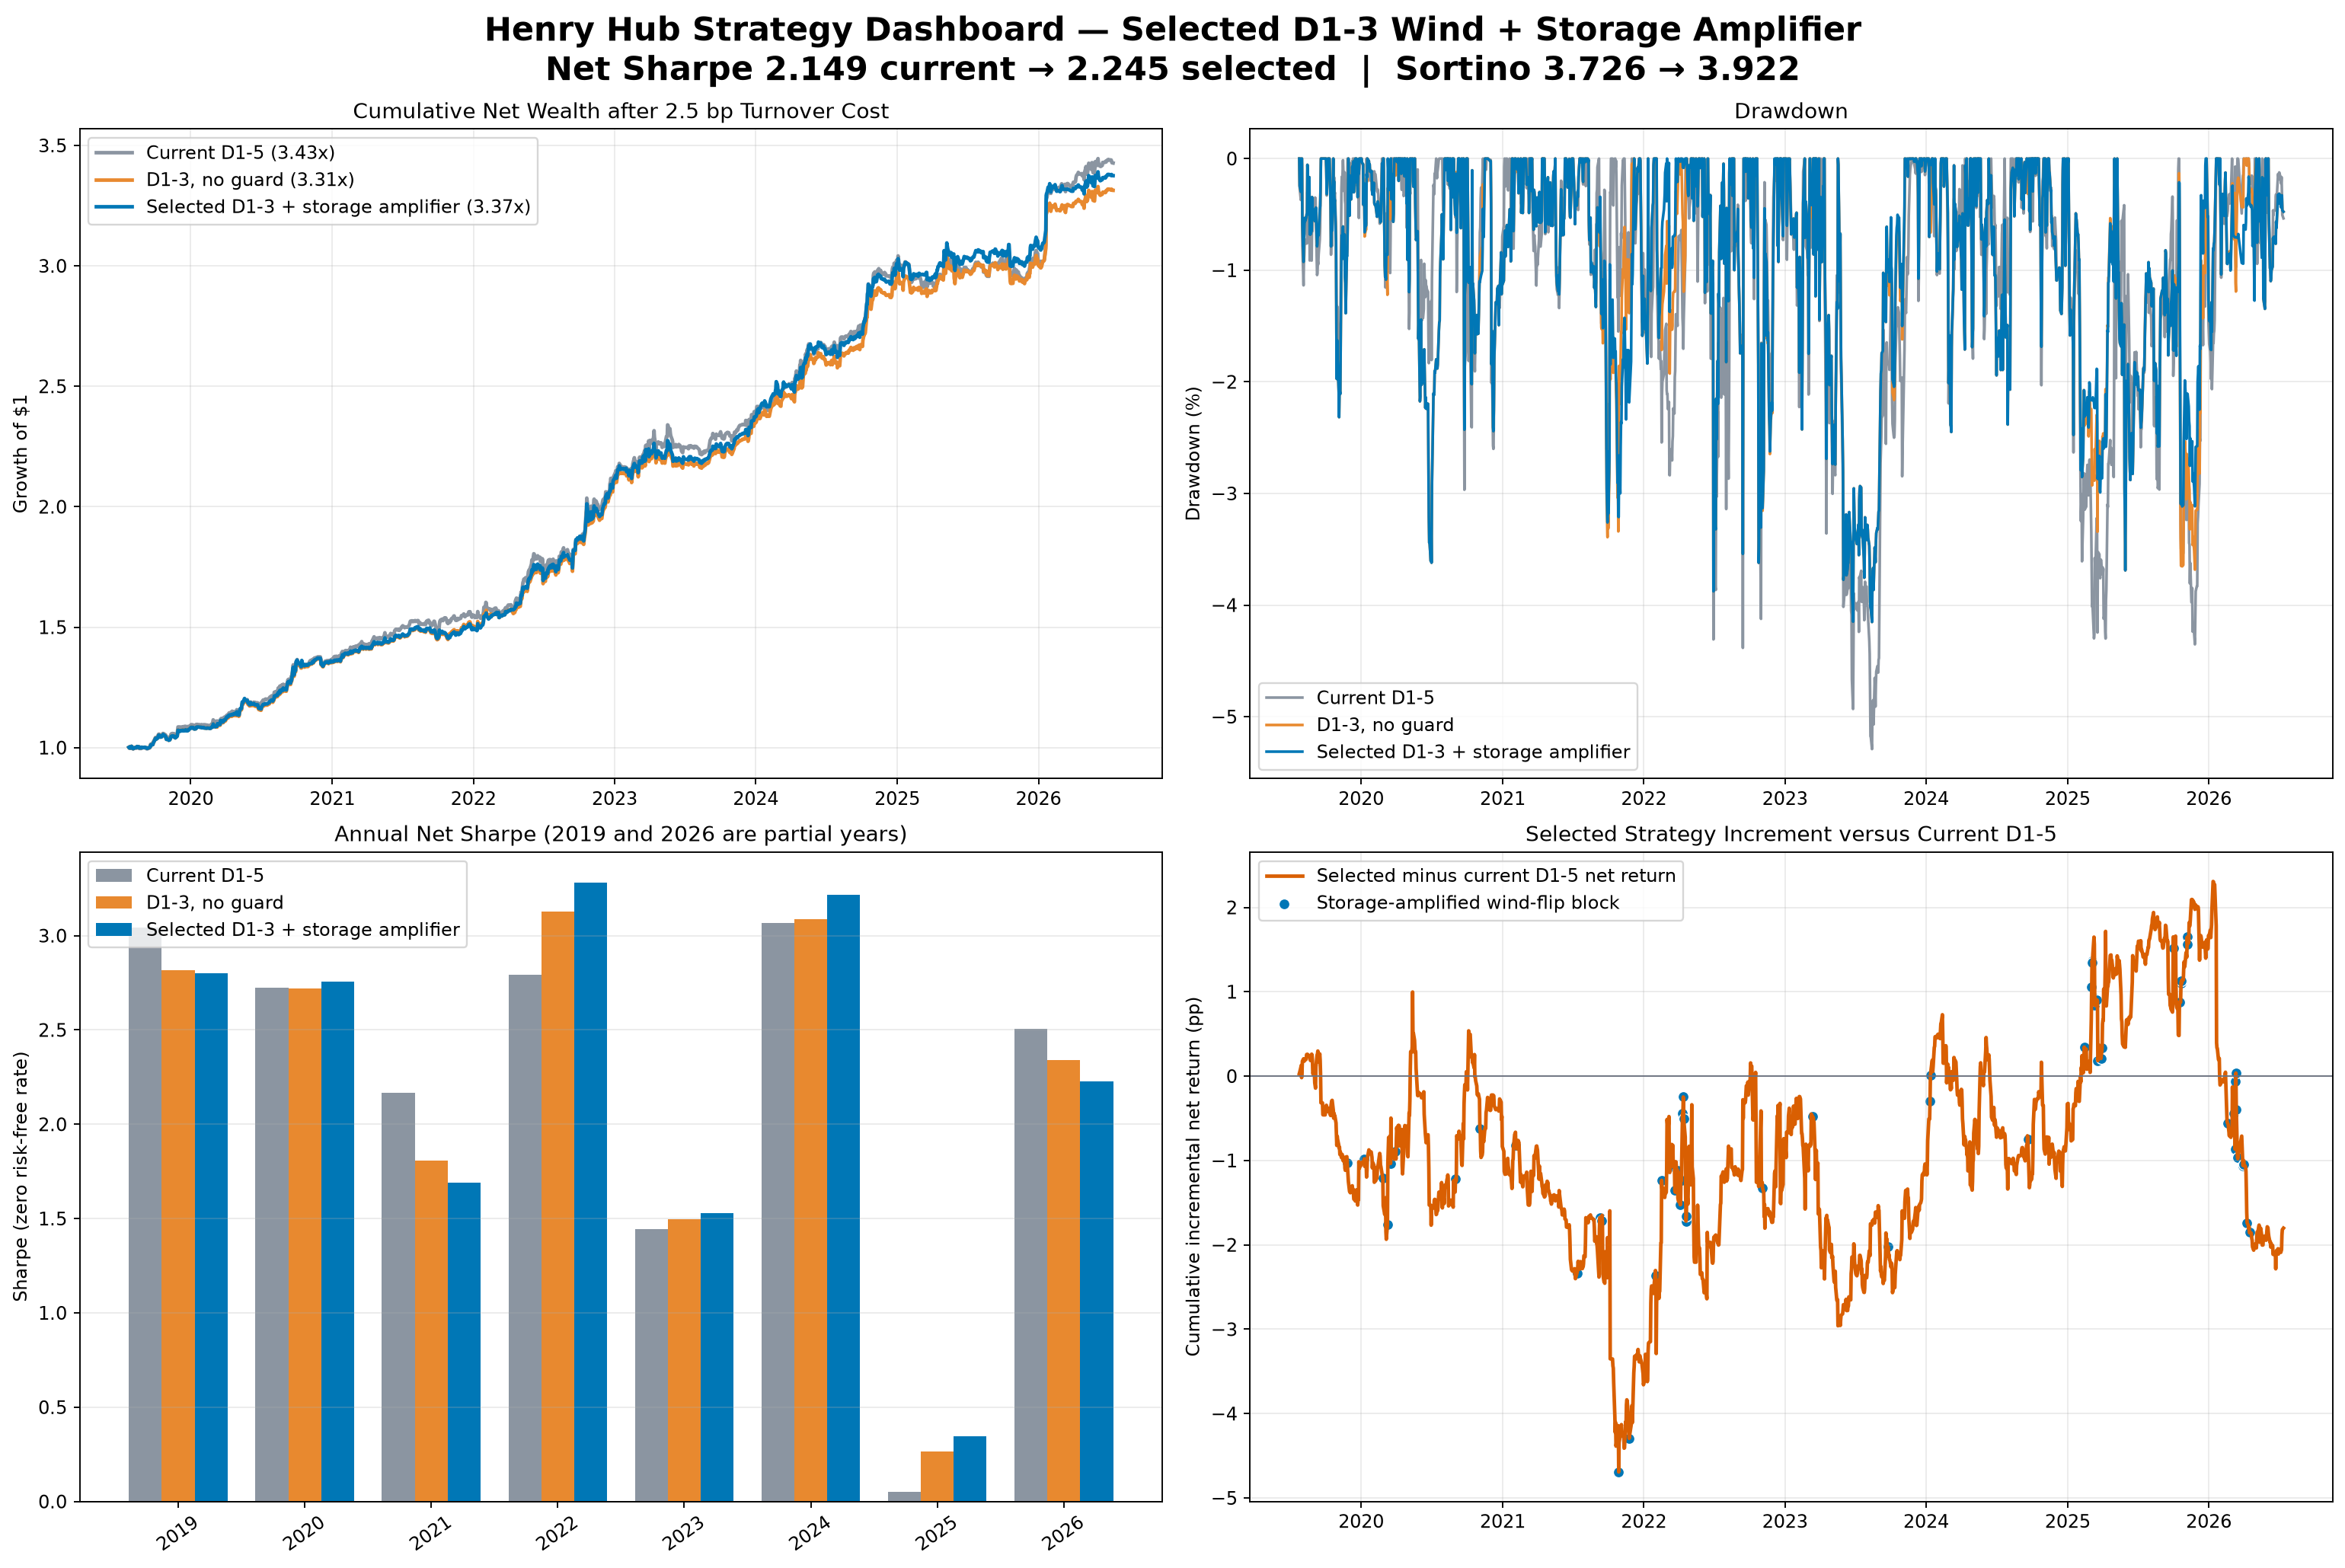
\includegraphics[width=\textwidth]{../results/experiments/d1_3_storage_amplified/latest_strategy_dashboard.png}
\caption{Selected D1--3 strategy dashboard.}
\end{figure}

The strongest conclusions are that renewable-generation conditions contain
incremental information, native-frequency standardization is necessary, and
regional storage is economically preferable to a purely national measure.
The largest unresolved weakness is historical-vintage quality rather than a
known mechanical date look-ahead.

\section{Model-Version Boundary}

The historical formal model contains South Central Total storage, CPC seasonal forecast
revision, capacity-weighted nonlinear wind shortfall, capacity-weighted PV
shortfall, a production-freeze control, a one-session lag, the fixed early
roll, and the 2.5 bps turnover cost.

The selected research version adds a fixed 10\% EIA-930 sleeve funded from
fundamentals: 40\% Central total non-gas generation shortfall and 60\% Florida
coal, nuclear, and water generation shortfall relative to demand. It also adds
a pure BSEE/Sabine short veto. It replaces the wind average from forecast days
1--5 with days 1--3 and adds a storage-amplified fast-shock direction guard.
Neither control can create or amplify a position. The nine internal fundamental
signals remain unchanged.

It excludes EBB pipeline overlays, weekend reopen trades, perfect-information
EIA experiments, direct observed weather, direct CPC forecast level, and macro
or market-price overlays. These exclusions prevent unstable or
publication-time-infeasible results from being mixed with the reported Sharpe.

\section{Economic Mechanism}

Cold winter weather raises heating demand; hot summer weather raises cooling
load and often gas-fired power burn. Forecast changes matter because futures
prices react before physical demand occurs.

Wind and solar displace gas generation when available. Expected renewable
shortfalls therefore raise expected power burn and are bullish natural gas.
Storage below normal, slower dry-gas production, stronger LNG exports, and
lower net-import availability also represent tighter U.S. balances.

South Central storage is particularly relevant because Henry Hub is located
in Louisiana and is connected to Gulf Coast production, LNG terminals, salt
storage, and major pipeline systems.

\section{Model Architecture}

Let the contemporaneous score be
\begin{equation}
S_t=w_{W,t}W_t+w_{wind,t}Wind_t+w_{F,t}F_t+w_{solar,t}Solar_t.
\end{equation}

After the one-sided production-freeze control produces $\widetilde S_t$, the
position is
\begin{equation}
P_t=\operatorname{clip}(\widetilde S_{t-1},-1,1).
\end{equation}

Net return is
\begin{equation}
r^{net}_t=P_t r^{fut}_t-0.00025\left|P_t-P_{t-1}\right|.
\end{equation}

\section{Causal Standardization and Data Timing}

Weekly and monthly values are standardized at their native release frequency
before forward-fill. This avoids treating one monthly release repeated across
approximately 20 trading days as 20 independent observations.

Weekly storage uses 104 releases with a 52-release minimum. Monthly production,
LNG, and trade variables use 60 months with a 36-month minimum. The current
observation is excluded from its own rolling reference distribution.

Weekly EIA storage for a week ending Friday becomes usable the following
Thursday. Monthly EIA reference month M becomes usable at the start of M+3 in
the conservative formal convention. GFS issue time is retained and the final
model adds a one-session lag.

\section{CPC Weather Module}

Only CPC seasonal forecast revision is active. CPC forecast level and observed
weather remain neutral zero slots:
\begin{equation}
W_t=\frac{\tanh(CPCRevision_t/2)+0_{level}+0_{observed}}{3}.
\end{equation}

The denominator remains three so removing two unstable factors does not
mechanically triple the surviving revision signal.

\section{Wind Module}

The factor uses GFS 80 m wind from the 00Z cycle at 28 representative
locations. The selected version aggregates forecast days 1--3; days 1--5 are
retained as the prior comparator. Wind is adjusted to hub height with
\begin{equation}
v_h=v_{80}\left(\frac{h}{80}\right)^{0.14}.
\end{equation}

The generic power curve has cut-in near 3 m/s, rated output from approximately
12 to 20 m/s, cosine derating from 20 to 25 m/s, and cut-out at 25 m/s. Power
is evaluated by location and valid time before capacity aggregation:
\begin{equation}
EstimatedWindCF_t=\frac{\sum_i Capacity_{i,t}P(v_{i,t})}
{\sum_i Capacity_{i,t}}.
\end{equation}

The gas-direction factor is
\begin{equation}
Wind_t=\tanh\left(\frac{Z^{causal}_{60}(1-EstimatedWindCF_t)}{2}\right).
\end{equation}

USWTDB capacity is reconstructed using commissioning year and excludes the
current issue year. The result is a regional availability proxy, not a
plant-level dispatch forecast.

The selected direction guard activates for a strong fast bullish shock or when
low South Central inventory coincides with a moderate fast bullish shock. Low
inventory cannot activate the guard alone. If the score without wind is
positive and bearish D1--3 wind would reverse it below zero, the guarded score
is set to zero. The guard cannot create or amplify exposure.

\section{Solar Module}

GFS downward shortwave radiation converts to six-hour energy as
\begin{equation}
E_{6h}=DSWRF\times\frac{6}{1000}\quad\text{kWh/m}^2.
\end{equation}

Surface energy is normalized by extraterrestrial horizontal radiation. A
simple cell-temperature proxy and efficiency adjustment are
\begin{align}
T^{cell}&=T_{2m}+0.025\,DSWRF,\\
\eta_T&=\operatorname{clip}\left[1-0.004(T^{cell}-25),0.75,1.10\right].
\end{align}

The capacity-weighted PV-availability shortfall receives a causal 60-issue
z-score and \code{tanh(z/2)} compression. The nominal 10\% allocation is scaled
by deterministic daylight and is funded from the fundamental block.

The module omits distributed capacity, detailed panel orientation, snow,
soiling, curtailment, outages, and hourly net-load value.

\section{Storage and Monthly Fundamentals}

South Central Total storage supplies level, one-week change, and four-week
change features. Each is compared with a prior-five-year same-week normal and
receives a negative causal z-score so tighter storage is bullish.

Active monthly features include low production YoY growth, LNG export YoY
growth, net-import supply, production MoM, LNG export MoM, and net-import-ratio
MoM change. Consumption YoY and MoM have zero weight because delayed nationwide
monthly consumption was too slow and overlapped strongly with weather.

\begin{table}[h]
\centering
\caption{Internal fundamental weights}
\begin{tabular}{lr}
\toprule
Component & Weight\\
\midrule
South Central low storage & 18.18\%\\
South Central one-week change & 9.09\%\\
South Central four-week change & 9.09\%\\
Low production YoY growth & 9.09\%\\
LNG export YoY growth & 9.09\%\\
Net-import supply & 9.09\%\\
Dry-production MoM & 9.09\%\\
LNG export MoM & 18.18\%\\
Net-import-ratio MoM change & 9.09\%\\
Consumption YoY and MoM & 0.00\%\\
\bottomrule
\end{tabular}
\end{table}

\section{Seasonal Allocation and Freeze Control}

Peak months use 45\% nominal legacy weather, 15\% wind, and 40\% fundamentals
before solar funding. Shoulder months use 22.5\% weather, 22.5\% wind, and 55\%
fundamentals. Solar receives its daylight-scaled nominal 10\% from fundamentals.

The current selected research version also funds a fixed 10\% EIA-930 sleeve
from fundamentals.
Peak months therefore retain 45\% weather and 15\% wind, with 10\% EIA-930,
0--10\% solar, and 20--30\% fundamentals. Shoulder months retain 22.5\%
weather and 22.5\% wind, with 10\% EIA-930, 0--10\% solar, and 35--45\%
fundamentals.

During November--March, if both the local freeze level and revision conditions
are met, the raw score cannot be negative. This is a one-sided safety control
against shorting during estimated production disruption.

\subsection{EIA-930 Central and Florida Generation Shortfalls}

The Central component aggregates realized non-gas generation across ERCOT,
MISO, and SPP. The Florida component measures coal, nuclear, and water
generation relative to demand across nine Florida respondents. A positive
shortfall indicates less non-gas generation and a potentially greater
requirement for gas-fired output. The fixed blend complements rather than
replaces the forward GFS wind and solar signals.

\subsection{BSEE/Sabine Pure Short Veto}

A worsening BSEE offshore shut-in accompanied by recent Sabine operational
context can set a conflicting core short to zero. The controller cannot create
a long, increase an existing long, or alter a non-conflicting position. The
selected D1--3 overlap contains six actual event-veto dates.

\section{Futures Roll and Costs}

The backtest switches from the contemporaneous C1 to C2 five full trading
sessions before the official last-trading-day convention. The 2.5 bps charge
applies to absolute position change. It does not separately model bid/ask,
market impact, or both legs of the mechanical monthly contract roll.

\section{Performance by Research Period}

\subsection{Historical Formal Baseline}

The following table belongs only to the unchanged 2017-start historical
artifact.

\begin{table}[h]
\centering
\begin{tabular}{lrrr}
\toprule
Period & Sharpe & CAGR & Maximum drawdown\\
\midrule
Development, 2017--2020 & 1.721 & 12.55\% & -4.39\%\\
Validation, 2021--2023 & 1.878 & 18.64\% & -5.12\%\\
First-look holdout, 2024+ & 1.407 & 12.97\% & -6.07\%\\
Full sample & \textbf{1.673} & \textbf{14.61\%} & \textbf{-6.07\%}\\
\bottomrule
\end{tabular}
\end{table}

\subsection{Current Selected Strategy on the Common Sample}

The current selected version combines D1--3 wind, the storage-amplified
fast-shock guard, the Central 40\% / Florida 60\% EIA-930 sleeve, and the
BSEE/Sabine pure short veto. All three rows use identical dates and inputs.
Showing unguarded D1--3 separately identifies the forecast-horizon effect
before the storage-amplified guard is applied.

\begin{table}[h]
\centering
\small
\begin{tabular}{lrrrrrr}
\toprule
Variant & Dev SR & Validation SR & First-look SR & Full SR & Full CAGR & Full DD\\
\midrule
Current D1--5 & \textbf{2.788} & 2.137 & 1.811 & 2.149 & \textbf{19.33\%} & -5.29\%\\
D1--3, no guard & 2.719 & 2.223 & 1.859 & 2.198 & 18.76\% & \textbf{-4.15\%}\\
\textbf{Selected D1--3 + amplifier} & 2.742 & \textbf{2.270} & \textbf{1.919} & \textbf{2.245} & 19.07\% & \textbf{-4.15\%}\\
\bottomrule
\end{tabular}
\end{table}

The D1--3 horizon provides most of the drawdown improvement. Adding the
storage amplifier raises full Sharpe from 2.198 to 2.245, validation Sharpe
from 2.223 to 2.270, and first-look Sharpe from 1.859 to 1.919. The selected
version remains weaker than D1--5 in the short development overlap and accepts
slightly lower full-sample CAGR.

\subsection{Current Selected Calendar-Year Results}

\begin{table}[h]
\centering
\begin{tabular}{lrr@{\qquad}lrr}
\toprule
Year & Net return & Sharpe & Year & Net return & Sharpe\\
\midrule
2019 partial & 7.87\% & 2.802 & 2023 & 12.22\% & 1.530\\
2020 & 25.71\% & 2.755 & 2024 & 26.90\% & 3.217\\
2021 & 10.00\% & 1.689 & 2025 & 2.40\% & 0.347\\
2022 & 41.58\% & 3.280 & 2026 partial & 9.58\% & 2.229\\
\bottomrule
\end{tabular}
\end{table}

All selected calendar years are positive in the revised-history backtest,
but 2021 and 2026 YTD have lower Sharpe than D1--5. The result is not uniform
annual dominance.

\subsection{2025 Weakness Review}

The historical formal artifact loses 3.60\% with a -0.533 Sharpe in 2025. On
the current common-sample calculation, D1--5 earns 0.36\% with a 0.050 Sharpe,
unguarded D1--3 earns 1.85\% with a 0.265 Sharpe, and the selected
storage-amplified D1--3 version earns 2.40\% with a 0.347 Sharpe. Its 2025
maximum drawdown is -3.69\%, versus -4.35\% for D1--5. The latest version
makes the year modestly positive, but 2025 remains weak rather than strong
evidence of edge.

\section{Look-Ahead Audit}

Implemented controls include retained GFS issue time, causal rolling windows,
native-frequency standardization, weekly and monthly release lags, lagged
capacity history, and a final one-session position delay.

Remaining risks are revised EIA series, reconstructed capacity histories,
incomplete release-timestamp archives, and settlement prices that do not prove
execution at the intended decision time. The model is release-lag-aware but not
fully vintage-pure.

\section{Perfect-Information Upper Bound}

Aligning final month-M production and consumption to month M and compressing
all fundamentals with \code{tanh(z/2)} raises current South Central full-sample
Sharpe to approximately 1.781 and improves drawdown to roughly -4.40\%.
Because those values were not available then, this is not tradable. It only
supports further research into timely regional production and consumption
estimates.

\section{Rejected or Deferred Experiments}

Weekend reopen flattening reduced current full Sharpe to 1.648. EBB receipt and
cycle-revision effects were regime dependent and based on short history.
Geopolitical, dollar, equity, curve, and other price overlays did not establish
stable incremental value. None is included in the formal model.

\section{Principal Limitations}

\begin{itemize}
  \item EIA and installed-capacity histories are revised rather than complete
        first-release archives.
  \item Wind omits OEM-specific curves, air density, wakes, icing, outages,
        congestion, and curtailment.
  \item Solar omits distributed PV, complete orientation/tracking, snow,
        soiling, clipping, and hourly net-load value.
  \item National monthly production and trade remain slow proxies for the Gulf
        Coast marginal balance.
  \item Settlement backtests do not include a complete liquidity, spread, and
        market-impact model.
  \item Later model choices viewed validation diagnostics, so the final model
        does not have a pristine untouched holdout.
\end{itemize}

\section{Recommended Next Work}

The highest priorities are to archive first-release EIA vintages, freeze
capacity snapshots, split renewable capacity by ISO, validate forecasted wind
and solar against EIA-930 or ISO generation, acquire timely power burn/LNG
feedgas/Gulf Coast production, extend EBB history, and reconstruct executable
prices and roll costs.

The next stage should improve point-in-time data and physical validation rather
than add more parameters to maximize historical Sharpe.

\section{Reproducibility}

\begin{itemize}
  \item Historical baseline notebook:
        \path{notebooks/01_final_south_central_strategy.ipynb}
  \item Selected notebook:
        \path{notebooks/07_d1_3_storage_amplified_strategy.ipynb}
  \item Evaluator: \path{naturalgas/evaluate_south_central_storage_strategy.py}
  \item Data manifest: \path{DATA_MANIFEST.md}
  \item Formal summary: \path{results/formal/summary.json}
  \item Weights: \path{results/formal/strategy_weights.csv}
  \item Period results: \path{results/formal/period_comparison.csv}
  \item Annual results: \path{results/formal/annual_comparison.csv}
  \item Selected evaluator:
        \path{naturalgas/evaluate_d1_3_storage_amplified_strategy.py}
  \item Selected summary:
        \path{results/experiments/d1_3_storage_amplified/summary.json}
  \item Selected dashboard:
        \path{results/experiments/d1_3_storage_amplified/latest_strategy_dashboard.png}
  \item Selected decision brief:
        \path{reports/d1_3_storage_amplified_strategy_brief.md}
\end{itemize}

The repository includes the factor builders, master-panel builder, pinned
generation manifests, and strict rebuild pipelines. Large source objects
remain in GCS; the supported build reconstructs the approved result from their
immutable archived generations. It does not claim that re-querying current
public APIs will return byte-identical historical data.

\section{Conclusion}

The strategy has a coherent economic mechanism spanning forward weather,
realized multi-fuel power generation, gas fundamentals, and bounded event-risk
control, with positive results across development, validation, and the
post-2024 period.

The current selected storage-amplified D1--3 version records 2.245 net Sharpe,
3.922 Sortino, 19.07\% CAGR, and -4.15\% maximum drawdown on the matched
2019--2026 sample. These figures supersede the earlier EIA-only selected
version in this report. The 1.673 Sharpe remains only the longer 2017-start
historical formal baseline.
The research direction deserves continued development. Formal deployment,
however, requires stronger point-in-time data, regional physical validation,
Gulf Coast local-balance information, and realistic execution auditing.

\end{document}
